\documentclass[../report.tex]{subfiles}
\begin{document} \chapter{Method} The method chapter subjects the reader to the framework used to qualitatively compare the algorithms with regards to the given dataset.

\section{Method Design Overview}
In order to generate results and compare the two different algorithms, a method design was planned and executed. The overall design is shown in \ref{fig:method} it includes the step of Preprocessing, Implementation, Result Generation and External Evaluation.


\begin{center}
  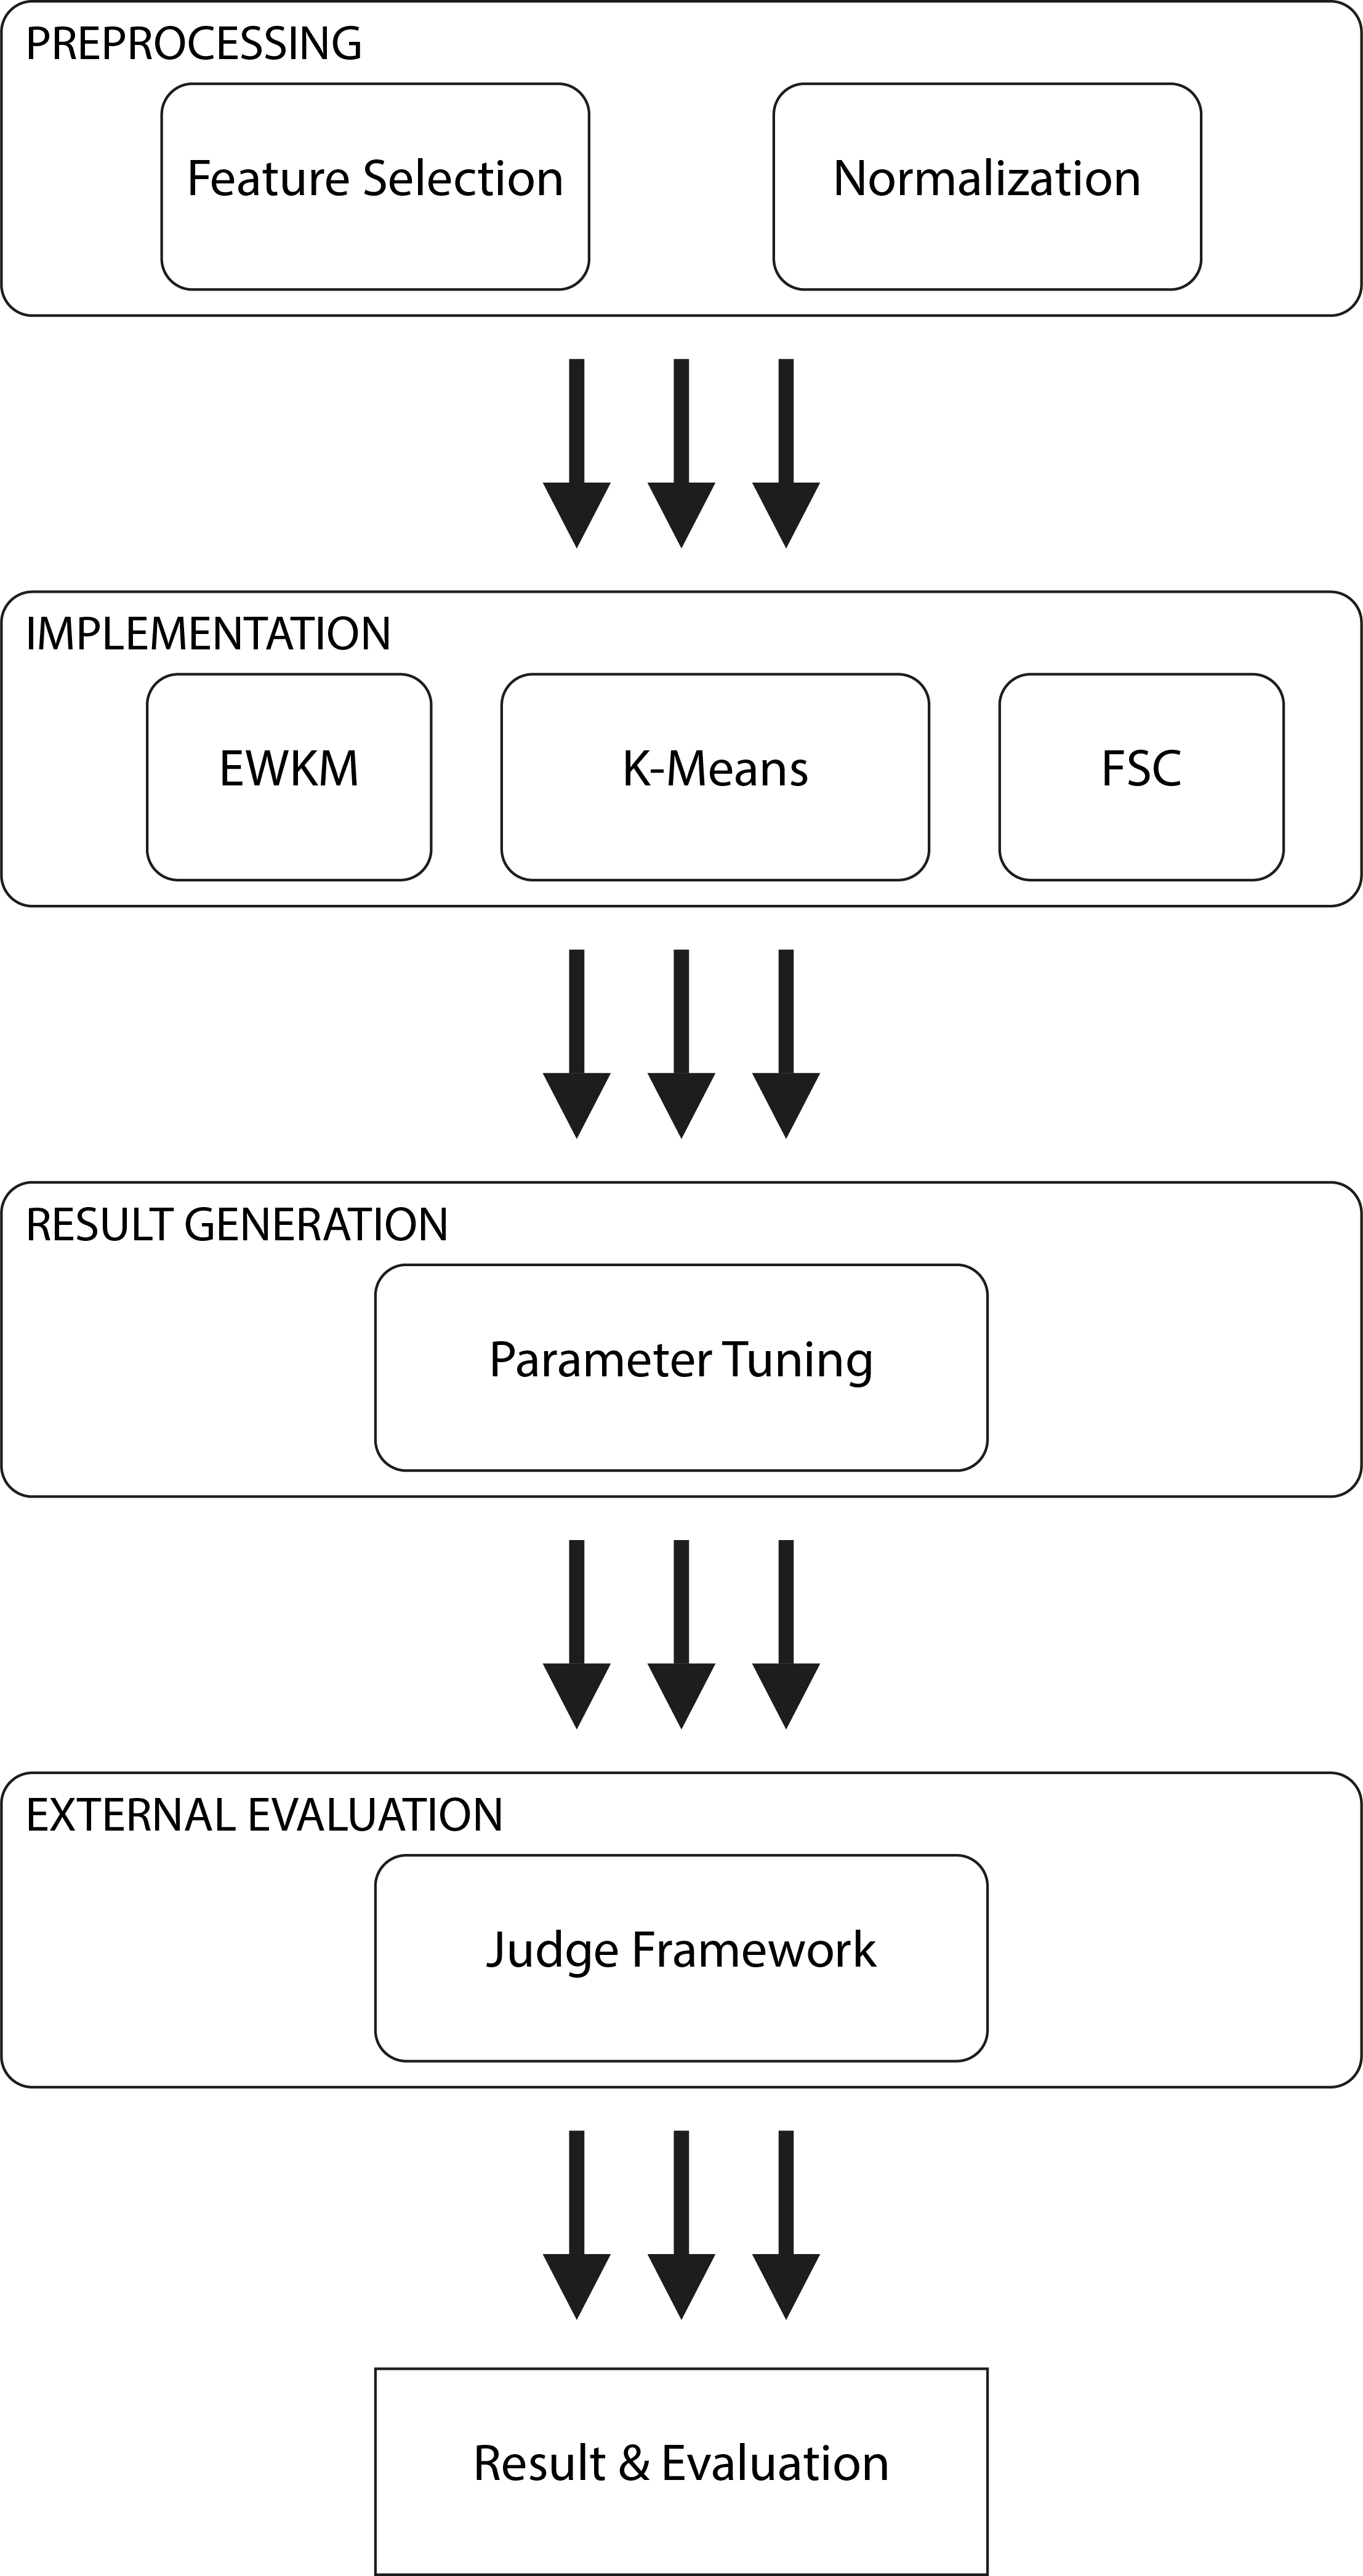
\includegraphics[width=0.31\textwidth]{Design}
  \captionof{figure}{\label{fig:method} Method Design}
\end{center}

% \begin{itemize}
%   \item Pre-Processing data
%   \begin{itemize}
%     \item Deciding on dataset size, and, feature-selection.
%   \end{itemize}
%   \item Picking an implementation of the algorithms and implementing needed functions.
%   \begin{itemize}
%     \item EWKM algorithm
%     \item K-means algorithm
%     \item Generating a distance matrix
%   \end{itemize}
%   \item Hyper-parameter tuning
%   \begin{itemize}
%     \item Deciding on $\gamma$
%     \item Deciding on $k$
%   \end{itemize}
%   \item Ranking Clusters
%   \begin{itemize}
%     \item Deciding on $\gamma$
%     \item Deciding on $k$
%   \end{itemize}
%   \item Evaluation Framework
%   \begin{itemize}
%     \item Silhouette
%     \item Purity
%     \item Expert Judging
%   \end{itemize}

% \end{itemize}

\section{Preprocessing}
\subsection{Dataset Properties}
% Clustering analysis will be made on a real-world-, high-dimensional- and, mixed-dataset.
The given dataset is a real-world-, high-dimensional- and, mixed-dataset. It is a set of \textit{songs} extracted from an company-internal music database. Each song is a vector of features --- each feature describes the song in a unique way. The vector consists of two different types of features; General metadata and metadata generated from an audio embedding.

The general metadata, includes attributes that predominantly identify the song without resulting to audio analysis. Features of the type were e.g. \textit{Album}, \textit{Artist}, \textit{Title} and \textit{Year of Origin}. The type also includes \textit{BPM} and \textit{Energy-feel}. These features include both numerical and categorical features --- features stored as strings can be converted to categorical data.

The second feature type is a 160-dimensional vector embedding --- with numerical values ranging through \begin{color}{red}{ -1 and 1 }\end{color} --- that characterizes the song through audio analysis. The embedding is generated through a neural network of auto-encoders, trained on the Mel-frequency cepstrum coefficients(MFCC)\cite{Paliwal2010}. The feature type is anonymous to humans, i.e. what exactly dimension 5 represents is unknown.

There is also feature named \textit{Genre} which holds a list of human-tagged genres that a song fits to. In total 33 genre tags exist in the dataset.
A minority of the songs do not hold a single genre.


\begin{color}{red}{
\subsection{MFCC}
To understand MFCC we need to first understand how humans perceive sound and how speech is created. Humans are more sensitive to frequency differences at lower frequencies compared to higher frequencies. The Mel-scale takes the differences in sensitivity into account by creating a logarithmic scale. Human speech is generated by the shape of the vocal tract. The shape determines what sound is created.
A power spectrum describes how much power is in the frequency component of a signal. The envelope of the power spectrum can be used to represent the shape of the vocal tract of the given audio. An MFCC represents the envelope \cite{Paliwal2010}. With the shape of the tract represented, generated phonemes can be determined of the vocals of the audio.
}\end{color}


\subsection{Feature-Selection and Normalization}
With a focus on tackling the problem of high-dimensionality, the choice was to use the numerical methods of \textit{EWKM}, \textit{FSC}, and, \textit{K-means}.
That left a restriction to only select numerical features as input. A hypothesis was that audio-embeddings can exclusively describe the songs in the dataset sufficiently. The dataset was therefore preprocessed to only include the subspace of embedding-features.

The \textit{genre} feature was additionally kept as an approximate ground truth label for further use in the external criteria.

As a next step in preprocessing, all features were normalized to the same variance, a way to make sure that all embeddings have the same impact on the algorithm.
For normalization Z-score was used ( See \ref{eq:z-score} ).


\begin{equation}
  \label{eq:z-score}
  z = \frac{x - \mu}{\sigma}
\end{equation}

\section{Implementation}
\subsection{EWKM Implementation}
The chosen EWKM algorithm is available in \textit{R and CSRAN} through the \textit{wskm} package \cite{wskm2014hz}. The source code is available for the public on github. The algorithm is implemented in $C$ and wrapped for $R$.

The implementation differs slightly in how $w_{lj}$ is calculated from the algorithm shown in \ref{eq:ewkm}. It includes additional normalization steps. Eq \ref{eq:newlambda} shows how $w_{lj}$ is updated in the given implementation. 

Another deviation from the original algorithm is how empty clusters are treated. In this implementation cluster center's are re-sampled if the originally picked centers result in empty clusters i.e. the algorithm is re-ran if empty clusters are occurring. Additionally a convergence value can be set by the user.
% restarts?

Per request of the stakeholder along with the author's familiarity with Python and Pandas DataFrame, the code was re-wrapped for Python using numpy-C-API \cite{numpy-c} --- allowing for the dataset to be sent in to the algorithm as a numpy array. The C-code was tweaked to not be dependent on R's \textit{unif\_rand() function}. The altered C-code along with the Python wrapping can be found in the attachments.... 

\begin{align}
  \lambda_{lj} &= \exp\bigg({\Big(\frac{-D_{lj}}{\gamma}\Big) - \max_{\forall{t} \in C_l}\Big({\frac{-D_{lt}}{\gamma}}\Big)}\bigg) \\
  \lambda_{lj} &= \max\bigg(\frac{\lambda_{lj}}{\sum_{t=1}^{m}{\lambda_{lt}}}, \frac{0.0001}{m}\bigg)\\
  \label{eq:newlambda}
  w_{lj} &= \frac{\lambda_{lj}}{\sum^{m}_{t=1}{\lambda_{ lt }}}
\end{align}

\subsection{FSC Implementation}
The FSC implementation was created by the thesis author and is based on the C-code of \textit{EWKM}. The methods of calculating cost, updating weights and updating cluster memberships were modified to correspond to the FSC algorithm as shown in \ref{eq:cost-fsc}, and \ref{eq:fsc}. $\gamma$ is replaced by $\beta$, and the small value of $\epsilon$ was set to $0.001$ as proposed in \cite{Gan2006}.

\subsection{K-means Implementation}
\textit{EWKM} is equivalent to \textit{K-means} when $\lim_{\gamma \to 0}$, although simply setting $\gamma = 0$ forces division by zero. As such it was simpler to use another package for \textit{K-means}. \textit{K-means} being a popular clustering algorithm, is widely available for Python. The PyClustering implementation of \textit{K-means} was used for this report \cite{Novikov2019}. The implementation was created in \textit{C++} and wrapped for Python.

\section{Result Generation: Parameter Tuning}


\subsection{Purity}

As stated above the \textit{genre} feature was kept. With it an external criteria could be created, the measurement of purity was combined with the feature to create a external criteria. The most dominant genre of each cluster was aggregated and divided by the total amount of songs in the dataset.

It is important to highlight the problem of only relying on this criteria to evaluate the results. A good song cluster does not have to be genre homogenic. A good cluster could hypothetically be Christmas music and hold multiple genres, this would then be discarded by the evaluation as a bad cluster. The evaluation was tehrefore not used, for the final evaluation. It was however, deemed as a suitable score for the processes of parameter tuning.

\subsection{Average Silhouette}

The internal criterion of average silhouette can be used for parameter tuning. Soft-subspace clustering requires the creation an asymmetric distance matrix, as the distance from \textit{Object A} to \textit{Object B} is dependent on the subspace weights of the cluster in which \textit{Object B} resides in.

1000 objects were sampled from the result to generate the asymmetric distance matrix. From there, the \textit{sklearn} package was used for average silhouette calculation.

\subsection{Tuning K - Amount of Clusters}

$k$ could have been decided on a smaller sample of the dataset, or through the use of a competitive learning strategy as discussed in the background. Due to the already relative small sample of the whole dataset and an algorithm that is linear in time it was decided to decide $k$ based on the results of the whole sample dataset with respect to the best $\gamma$ in regards to the cost function.

$k$ was checked for the values of 50, 100, 500, 1000 and compared through the \begin{color}{red}{average silhouette} \end{color}. It was not important for this project to get the exact best $k$ rather what approximately range $k$ should be picked. The minimum of $50$ clusters was based on that the number of genres in the dataset was 33, and generated clusters should at least be as specific as a genre label. On the other side of the scale, 1000 was decided as the maximum amount of clusters as more would result in an average less than 50 songs per cluster. Additionally, if you were to scale the dataset to $50*10^7$ songs, more cluster would translate into more expensive computations.


\subsection{EWKM}
$\gamma$ is a hyper-parameter of EWKM. In short, $\gamma$ determines the likeliness to cluster on more or less features. For any given dataset the ideal $\gamma$ can vary. An ideal $\gamma$ is found when there is no other $\gamma$ value that can result in a lower cost.

The EWKM algorithm does not try to maximize the inter-cluster distance between clusters. The best $\gamma$ in regards to a minimized intra-cluster distance and a maximized inter-cluster distance --- Which can be expressed by the average silhouette --- does not have to equal the $\gamma$ which produces the lowest cost function. To attest for the difference the result of the best $\gamma$ in regards to the average silhouette was compared with the best $\gamma$ in regards to the cost function. Discarding any of the two before comparison could lead to sub-optimal results.

$\gamma$ was chosen by iteratively testing different values of the parameter as an input for the algorithm, from small ($1 * 10^{-3}$) to large ($\gamma = 3$).
The results on the sample dataset -- of the different $\gamma$ values --- was compared in regards to \color{red}{silhouette and purity.}



% High $\gamma$ values were found to force an immediate convergence as the negative shannon entropy became larger than the euclidean distance part of the cost function. 

% The $\gamma$ with the lowest silhouette was then tweaked to see if a lower cost function could be obtained. 

\subsection{Ranking songs and clusters}
A distance array --- based on the subspace distance measure of the algorithm ---- between each point and the cluster center in which the point is a member in was generated.  Songs within a cluster could then be ranked by the ascending distance to the center. Clusters could also be ranked by representing the cluster \textit{"goodness"} through the ascending average distance of the songs. Here, it was deemed that good clusters should not be picked based on genre purity.

The ranking allowed for a cutoff in songs and clusters i.e. the top 10 clusters could be chosen and the clusters and from there a cluster could be shrank by only picking songs with a certain distance to the cluster center.

\subsection{Judge Evaluation}
\color{red}{
Purity using the genre as benchmark, assumes that a good cluster is genre coherent. While it could be true, a good cluster could be cross-genre such as Christmas music. To adhere}

A website page was created where judges could listen to songs of a cluster and rank it. Each cluster could be ranked by cohesion (similarity between songs) and novelty (if the cluster was generating a new type of mini-genre) on a scale 1-10.

Ten songs were sampled on a half-norm distribution --- based on the songs distances. A blind test was created, in which five songs of each algorithm was picked. To allow a reference point, three clusters were generated from previously created playlists. Judges were to choose the novelty and cohesion of each cluster.

The website was built in django and bootstrap. A screenshot can be found in appendix....




% Songs and clusters were sorted by generating the distance between each point and the center of the cluster the point was situated in.  
% Diffrent $\gamma$'s were chosen with parameter was found by 
% for setting $\gamma$. A too high $\gamma$ results in a total entropy larger than the total distance. A $\gamma$ set too low resulted in slow convergence and a high cost function. The parameter was tuned by iteratively running the clustering method on multiple $\gamma$'s and choosing the $\gamma$ which results in the lowest cost function.
% '

\end{document}

